\documentclass{article}

\usepackage{graphicx}
\usepackage{tikz}
\usepackage{tikzsymbols}
\usetikzlibrary{calc,patterns,shapes.geometric}
\pagestyle{empty}
\usepackage[margin=0pt]{geometry}
\geometry{papersize={14in,12in}}

\def\centerarc[#1](#2)(#3:#4:#5){\draw[#1] ($(#2)+({#5*cos(#3)},{#5*sin(#3)})$) arc (#3:#4:#5);}

\begin{document}
	\begin{figure}
		\centering
		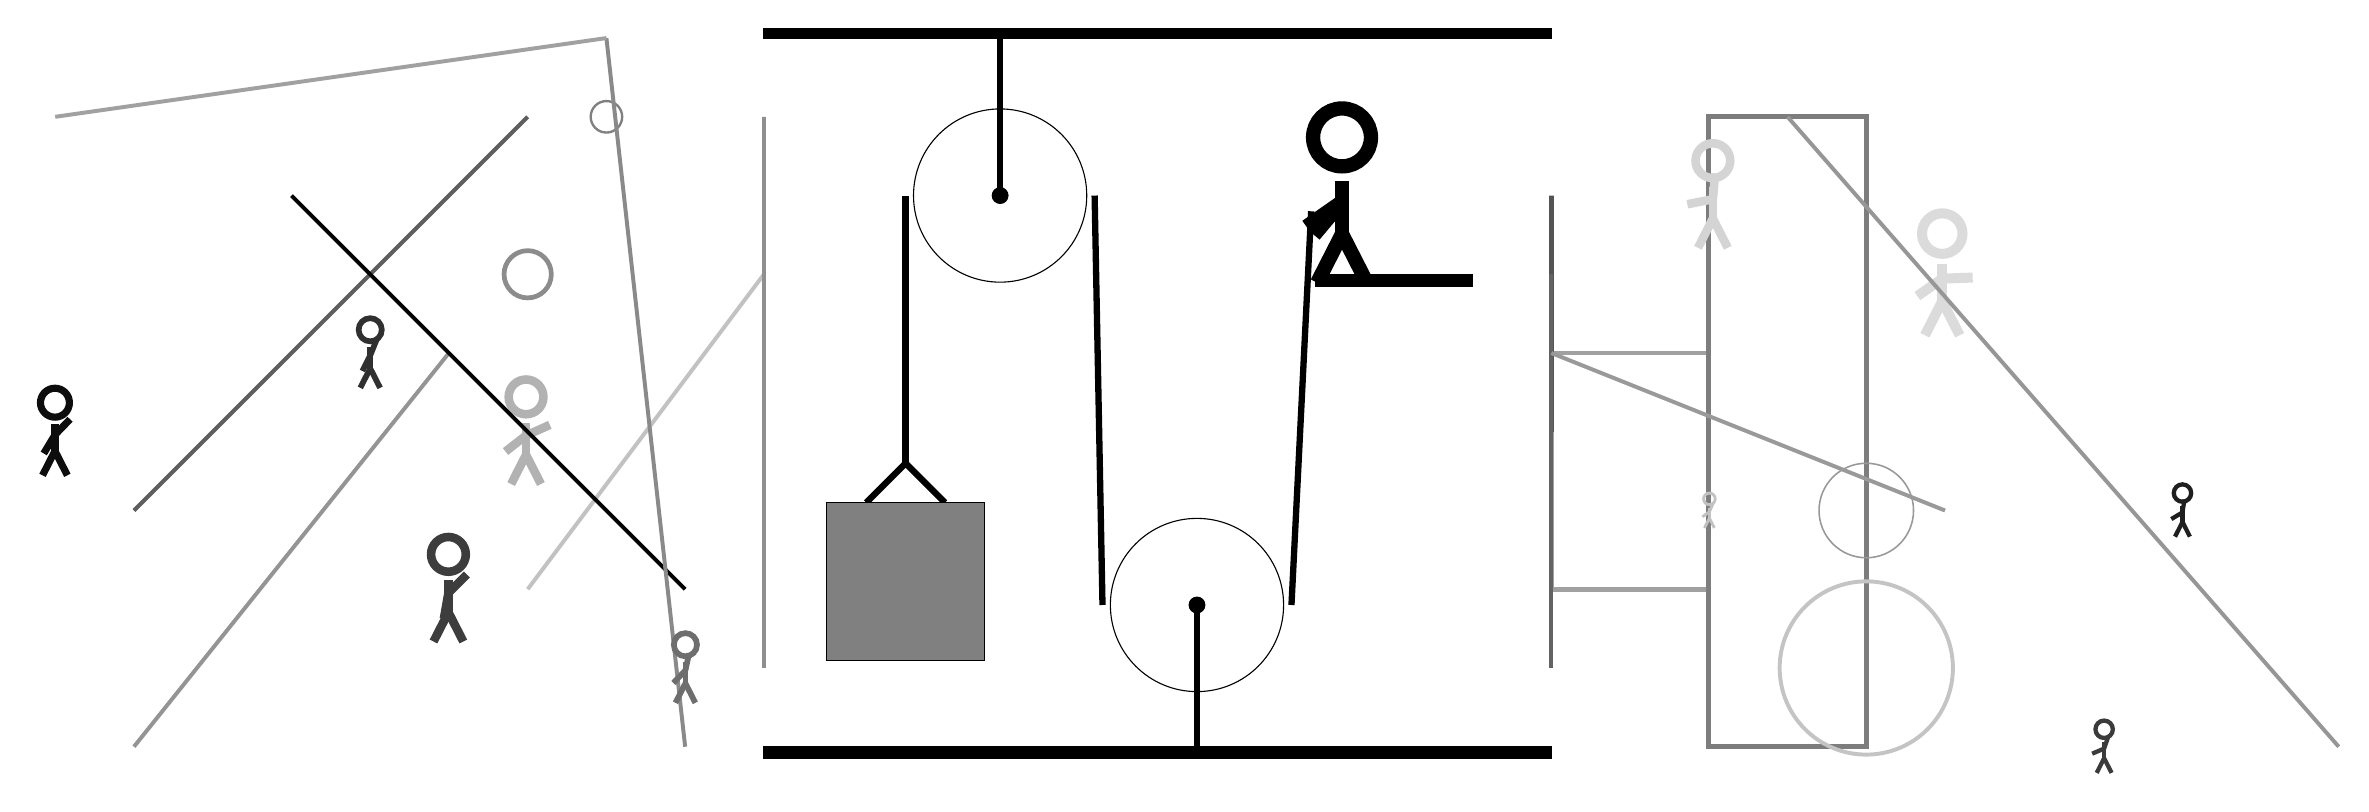
\begin{tikzpicture}
			%%%%% START %%%%%
			
			\draw[fill=black] (-2, 9) rectangle (8, 9.125);
			
			\draw (3.5, 1.8) circle (1.1);
			\draw[fill=black] (3.5, 1.8) circle (0.1);
			\draw[line width=0.8mm] (3.5, 1.8) -- (3.5, 0);
			
			\draw (1, 7) circle (1.1);
			\draw[fill=black] (1, 7) circle (0.1);
			\draw[line width=0.8mm] (1, 9) -- (1, 7);
			
			\draw[line width=0.8mm](-0.7, 3.1) --  (-0.2, 3.6) -- (0.3, 3.1);
			\draw[fill=black!50] (-1.2, 3.1) rectangle (0.8, 1.1);
			
			\draw[line width=0.8mm](-0.2, 7) -- (-0.2, 3.6);
			\centerarc[line width=0.8mm](1, 7)(180:0:1.2000000000000002)
			\draw[line width=0.8mm](2.2, 7) -- (2.3, 1.8);
			\centerarc[line width=0.8mm](3.5, 1.8)(180:360:1.2000000000000002)
			\draw[line width=0.8mm](4.7, 1.8) -- (4.95, 6.8);
			
			\node at (5.3, 7) {\Strichmaxerl[10][35][-130]};
			\draw[fill=black] (5, 6) rectangle (7, 5.85);
			
			\draw[line width=0.5mm, color=black!42](-6, 5) -- (-10, 0);
			
			\draw[line width=0.5mm, color=black!24](-5, 2) -- (-2, 6);
			\node[line width=0.5mm, color=black!77] at (15, 0) {\Strichmaxerl[3][23][71]};
			\draw[line width=0.6mm, color=black!37] (8, 2) rectangle (10, 5);
			\draw[line width=0.6mm, color=black!51] (10, 0) rectangle (12, 8);
			
			\draw[line width=0.6mm, color=black!67] (8, 7) rectangle (8, 4);
			\node[line width=0.3mm, color=black!30] at (-5, 4) {\Strichmaxerl[6][38][24]};
			\draw[line width=0.5mm, color=black!61](8, 6) -- (8, 1);
			\node[line width=0.3mm, color=black!88] at (16, 3) {\Strichmaxerl[3][31][81]};
			
			\draw[line width=0.5mm, color=black!63](-5, 8) -- (-10, 3);
			\node[line width=0.7mm, color=black!24] at (10, 3) {\Strichmaxerl[2][36][66]};
			
			\draw[line width=0.5mm, color=black!99](-3, 2) -- (-8, 7);
			\node[line width=0.4mm, color=black!14] at (13, 6) {\Strichmaxerl[7][35][2]};
			
			\draw [line width=0.5mm, color=black!23](12, 1) circle (1.1);
			\node[line width=0.5mm, color=black!17] at (10, 7) {\Strichmaxerl[6][11][85]};
			\node[line width=0.7mm, color=black!76] at (-6, 2) {\Strichmaxerl[6][80][45]};
			\draw[line width=0.5mm, color=black!41](11, 8) -- (18, 0);
			\draw [line width=0.3mm, color=black!50](-4, 8) circle (0.2);
			\draw[line width=0.5mm, color=black!46](-4, 9) -- (-3, 0);
			\draw[line width=0.6mm, color=black!44] (-2, 8) rectangle (-2, 1);
			\node[line width=0.5mm, color=black!95] at (-11, 4) {\Strichmaxerl[5][59][46]};
			\node[line width=0.4mm, color=black!57] at (-3, 1) {\Strichmaxerl[4][46][78]};
			
			\draw[line width=0.5mm, color=black!37](-4, 9) -- (-11, 8);
			\draw [line width=0.2mm, color=black!40](12, 3) circle (0.6);
			\draw[line width=0.5mm, color=black!40](8, 5) -- (13, 3);
			
			\draw [line width=0.6mm, color=black!45](-5, 6) circle (0.3);
			\node[line width=0.5mm, color=black!81] at (-7, 5) {\Strichmaxerl[4][63][68]};
			\draw[line width=0.2mm, color=black!25] (9, 0) rectangle (9, 0);
			\draw [line width=0.7mm, color=black!93](-11, 5) circle (0.0);
			
			
			\draw[fill=black] (-2, 0) rectangle (8, -0.15);
			
			%%%%% END %%%%%
		\end{tikzpicture}
	\end{figure}	
\end{document}